%=========================================================================
\documentclass[11pt,twoside,a4paper]{article}
\usepackage[english]{babel}
\usepackage{a4wide,times}
\usepackage{graphicx}
\usepackage{caption}
\usepackage{subcaption}
\title{Serial Peripheral Interface report}
\author{
Made by\\
Job Tijhuis, 4275756\\
Wietse Bouwmeester, 3456738\\
}
\date{26 November 2014}
\begin{document}
\maketitle
\thispagestyle{empty}
\vspace{30 mm}
\begin{center}
\Large \bf 
Abstract
\end{center}
This document describes the contents a design report for the module assignment of the EPO-3 project. 
It can be used a template for writing this report. 
Here you should give a summary of the report.
\clearpage

\tableofcontents
\clearpage

\section{Introduction}
Tell something about the context of this report.

\section{Specification}
Give the literal design specification of the client.

\section{Design}
In the specifications it is given that communication is to go according to the SPI de facto-standard. SPI does not define what the communication will be, but it does define the way the data is transferred. The SPI standard defines two communication lines: one from the master to the slave and one from the slave to the master. These lines are connected to shift registers where the outgoing line is connected to the most significant bit and the incoming to the least significant bit. The third line is a clock signal which tells the slave when to sample the line and when to shift its shift register. Since the shift register is such an integral part of SPI it was decided to separate the design in two parts: the shift register and a control system based on a Finite State Machine which controls when the register shifts and when the slave clock will be on. Because it is also important that the transmission stops after all eight bits have been transferred there is also a counter which counts the slave clock, this information is then used by the control.

\begin{figure}[htp!]
\center
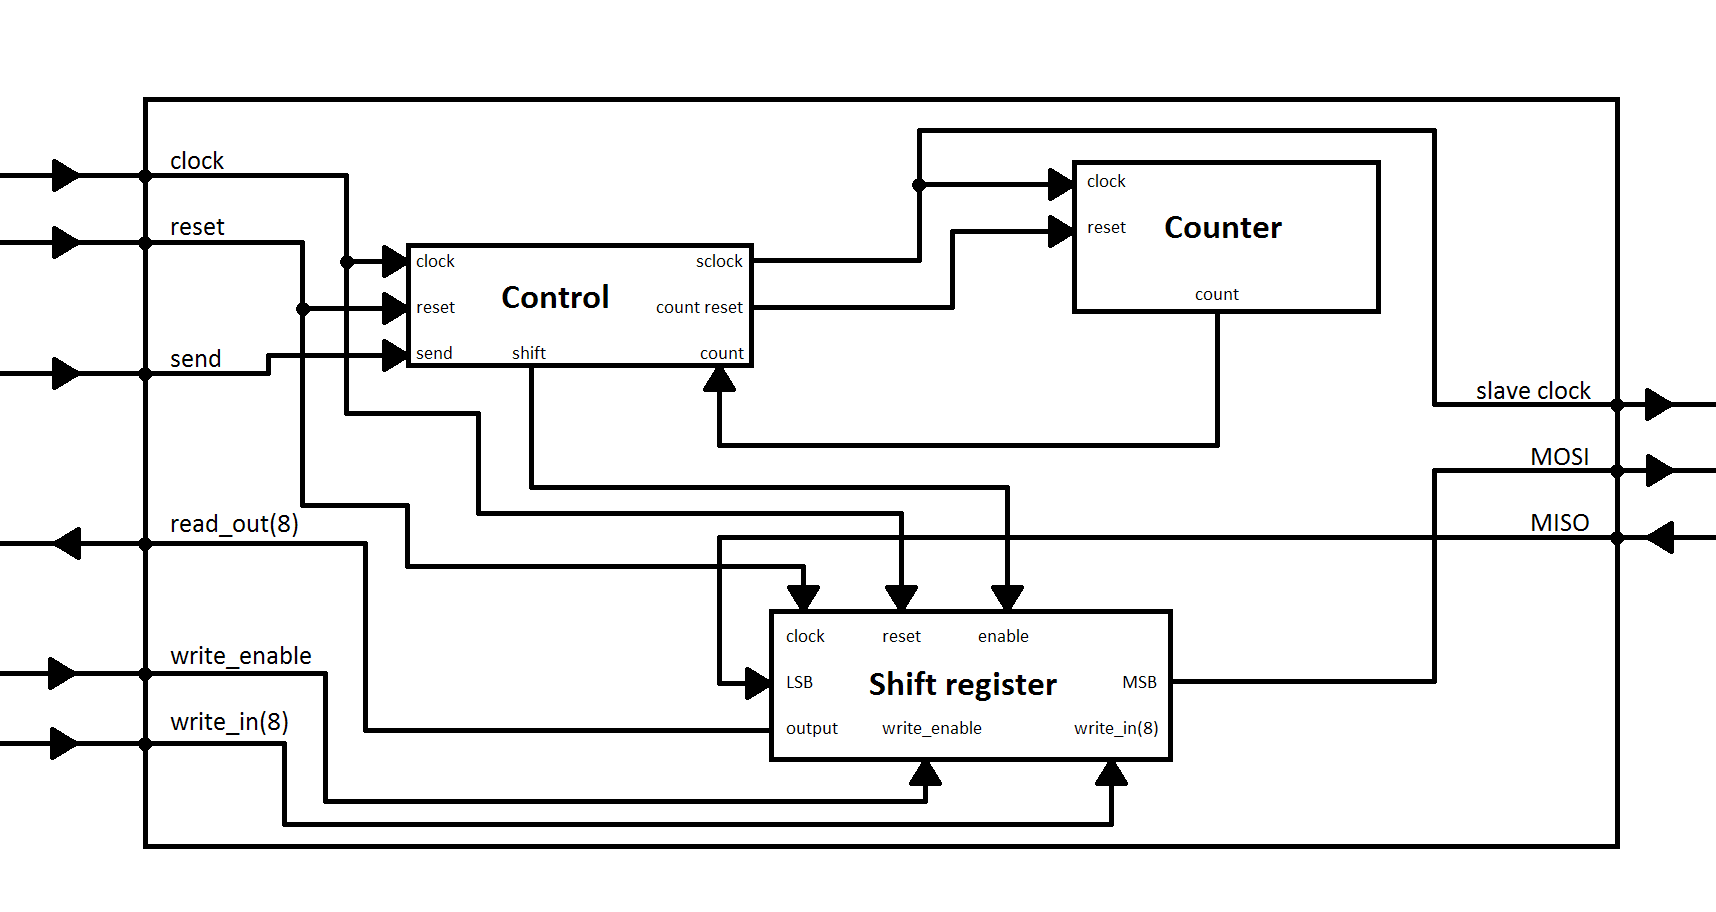
\includegraphics[width=14cm]{./spi_diagram}
\caption{Diagram of SPI circuit}
\label{spi-structure}
\end{figure}

\subsection{Control}
Control is a FSM and has three states: the reset state in which it will be once it is reset, the idle state in which it is when not shifting and to which it will return once all eight bits have been shifted and the shifting state in which it will actually shift the bits out/in. The VHDL implementation is the implementation of the finite state diagram in figure \ref{control-fsm}.
The output in the different states is as in figure \ref{control-states}.

\begin{figure}
\centering
\begin{minipage}{.5\textwidth}
  \centering
  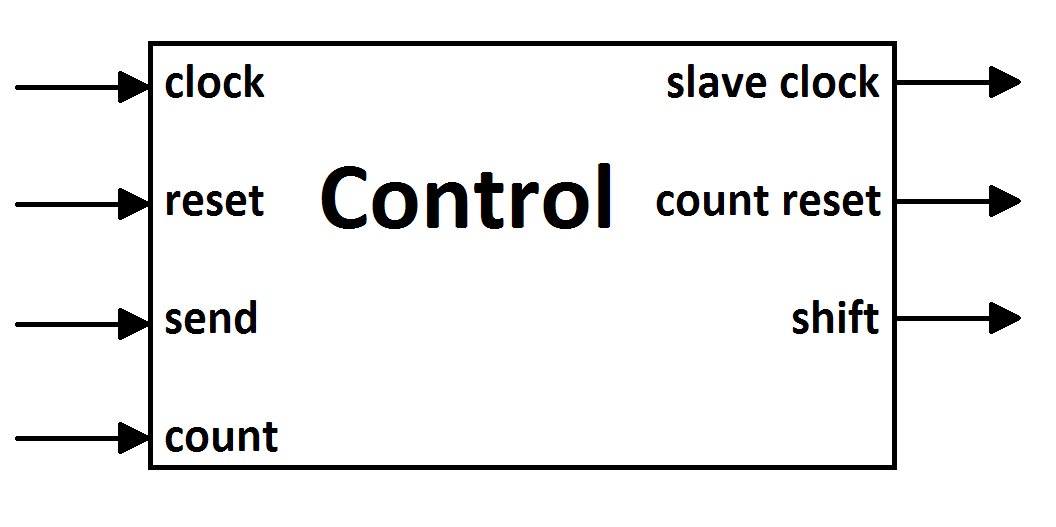
\includegraphics[width=7cm]{./control_diagram}
  \captionof{figure}{Diagram of Control}
  \label{control-diagram}
\end{minipage}%
\begin{minipage}{.5\textwidth}
  \centering
  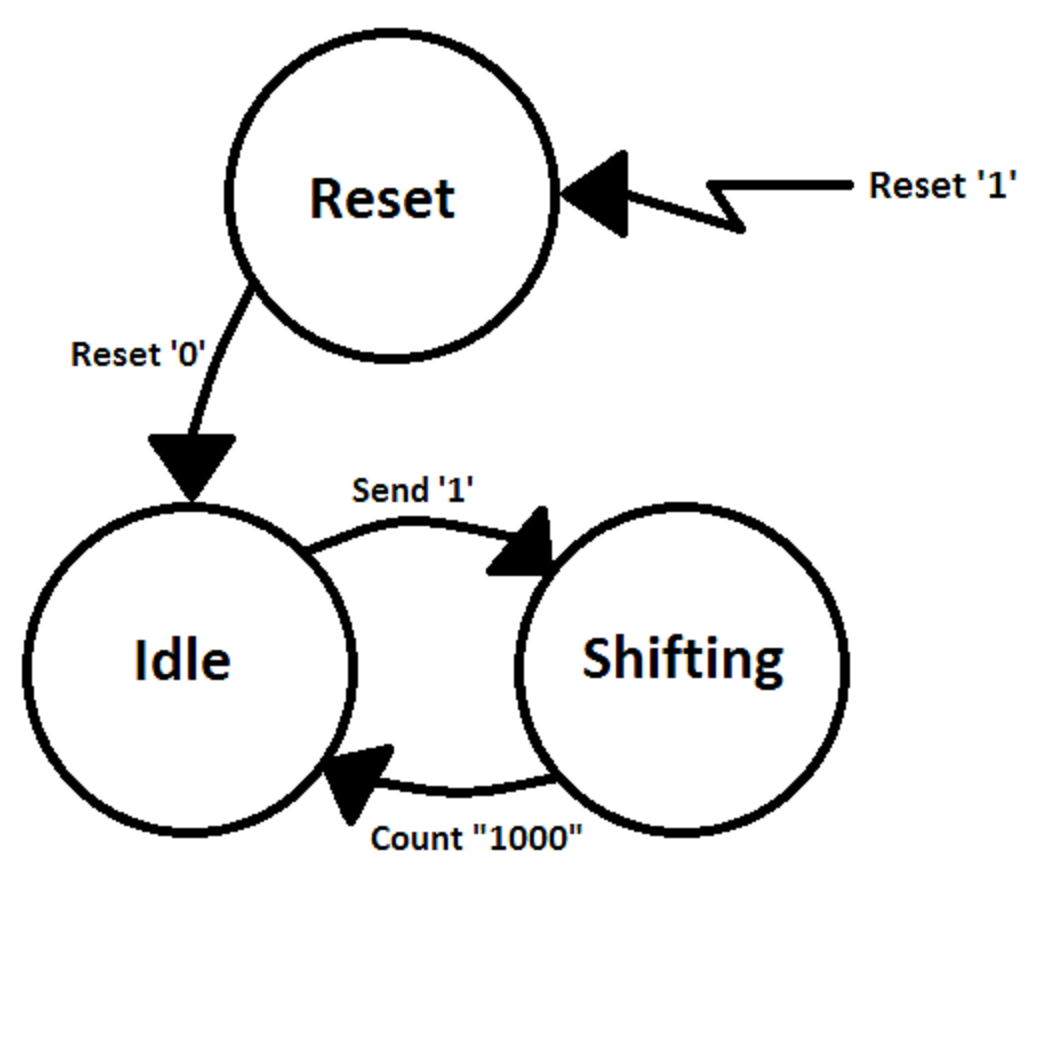
\includegraphics[width=5cm]{./control_fsm}
  \captionof{figure}{State diagram of Control FSM} 
  \label{control-fsm}
\end{minipage}
\end{figure}

\begin{figure}
\begin{center}
    \begin{tabular}{ | l | l | l | l |}
    \hline
    State & Slave clock & Count reset & Shift \\ \hline
    Reset & 0 & 1 & 0 \\ \hline
    Idle & 0 & 1 & 0 \\ \hline
    Shifting & not clk  & 0 & 1 \\
    \hline
    \end{tabular}
\end{center}
\caption{Control FSM states}
\label{control-states}
\end{figure}

\subsection{Shift register}
Incomplete
\subsection{Counter}
Incomplete
\begin{itemize}
\item
Block description with inputs and outputs.
\item
Possible subdivision into sub-blocks.
\item
One or more Finite State Diagrams, if appropriate.
\item
VHDL behaviour description(s).
\end{itemize}

\section{Results}
Tell about the results:
\begin{itemize}
\item
Simulation results for the VHDL top-level description.
\item
Layout results.
\item
Switch-level/Spice simulation results for the extracted circuit.
\end{itemize}

\section{Conclusions}
Does the design meet the specifications?
Is there something that can be improved?

\begin{thebibliography}{9}
\bibitem{labelboek1}
Author1, 
Book1, 
Publisher, 
year.
\bibitem{labelTitel}
Author1, 
Title, 
Magazine, 
Vol. 1, 
Nr. 1, 
year, 
pp. 12-15.
\bibitem{labelWeb}
Webpages title, 
http link, 
accessed on 19 sep. 2013.
\end{thebibliography}
\end{document}
